\chapter{Experimental Evaluation}
\label{ch:experiments}

This chapter evaluates the proposed Distributed Multimodal Sensing-Assisted
Beam Management framework, denoted by DMSA-BM.  The evaluation follows the
information flow established in Chapter~\ref{ch:methodology}.  Distributed
multimodal observations first support target-level detection and beam
prediction.  Target-to-user association and current-track observation then
determine whether a sensing-derived CSI-RS candidate set may be used.  The
resulting measurement decision is finally evaluated through average effective
user rate and CSI-RS overhead.  This organisation separates learning-level
evidence from its communication consequence and avoids interpreting
beam-prediction accuracy alone as a rate improvement.

\section{Dataset and Experimental Setup}
\label{sec:experiments-dataset}

\subsection{Multimodal Simulation and Data Generation}
\label{subsec:experiments-data-generation}

The experiments use a simulated multimodal V2I dataset comprising synchronised
multiview camera images, BS-local ISAC point clouds, vehicle annotations,
trajectories, and ray-traced channels.  These observations are organised into
target-BS-centred sensing samples and temporally aligned beam-management
episodes.

At a sensing epoch, the target BS receives its local camera observation, camera
observations from neighbouring sensing nodes, and a BS-local ISAC point cloud.
These inputs form the target-BS-centred multimodal observation used by the
perception network.  Each beam-management episode couples these observations to
the corresponding link evolution, beam labels, and vehicle trajectories.  The
perception, association, measurement, and resource-accounting stages therefore
operate on a common scene instance, while online decisions exclude ground-truth
VUE identities.

A sensing sample is indexed by environmental condition, sensing instant, and
target BS.  Link-level labels additionally identify the corresponding VUE for
supervision and evaluation.  The 48-beam SSB codebook and 192-beam CSI
codebook are linked through their parent relation.  The perception network
produces a 192-way beam-class posterior for an observed physical target.  Its
ranking is used to score association hypotheses and to reduce the CSI-RS
candidate set; it is neither a UE identifier nor a direct service-beam decision.

\subsection{Scenarios and Data Partitioning}
\label{subsec:experiments-scenario}

The data contain a four-BS roadside scenario under the \emph{Clear},
\emph{Rain/Fog}, and \emph{Night} conditions.  Each target BS serves a local
region and receives complementary observations from neighbouring sensing nodes.
Mutually disjoint training, validation, and test partitions are used throughout
the learning and system-level evaluations.  Target tracks and
target-to-user associations are maintained locally at each target BS; the
experiments do not assume a global identity that persists across serving cells.

\subsection{Communication Configuration}
\label{subsec:experiments-communication-configuration}

All system-level comparisons use a common radio configuration with a 100-ms
SSB periodicity, a 20-ms CSI-RS periodicity, and the 48-beam SSB and 192-beam
CSI-RS codebooks defined in Chapter~\ref{ch:system-model}.  The compared
policies also share the same ray-tracing segments, Doppler evolution, transmit
power, noise model, regularised zero-forcing processing, and resource
accounting.  The resulting communication model is a 5G NR-oriented abstraction
at the beam-measurement level rather than a PRB- and RE-level protocol model.

In the Rain/Fog condition, the association-margin threshold is fixed at
\(\tau_{\mathrm{margin}}=0.10\).  Because this operating point was selected
for the Rain/Fog test condition, the corresponding results characterise that
operating point rather than independent out-of-sample generalisation.

\section{Evaluation Methodology}
\label{sec:experiments-metrics}

\subsection{Detection and Beam-Prediction Metrics}
\label{subsec:experiments-learning-metrics}

Target detection is evaluated by AP@2m and Recall@2m.  The distance qualifier
requires a predicted target to lie within 2~m of its reference target, thereby
making the availability of a useful target-level observation explicit.  For
matched detections, Beam Top-1@2m and Beam Top-4@2m quantify whether the
strongest-beam class is retained by the predicted ranking.  The Top-4 power
ratio reports the fraction of reference link energy captured by the four
highest-ranked CSI beams.  It measures candidate-set utility, not calibration of
the beam-class posterior as a physical power distribution.

\subsection{Communication Metrics}
\label{subsec:experiments-system-protocol}

The system metric is the average effective user rate,
\begin{equation}
\bar{R}_{\mathrm{eff}}
 =
 \frac{1}{N}\sum_{n=1}^{N}
 \frac{1}{|\mathcal{U}_b[n]|}
 \sum_{u\in\mathcal{U}_b[n]}R_{b,u,n}^{\mathrm{eff}},
\label{eq:experiments-effective-rate}
\end{equation}
where \(N\) is the number of evaluated communication cycles and
\(R_{b,u,n}^{\mathrm{eff}}\) includes the resource effects of control, SSB,
CSI-RS, and data transmission at cycle \(n\).  The definition therefore compares
candidate-measurement policies after their communication overhead has been
accounted for.

The accompanying operational metrics are CSI-RS overhead, sensing-use ratio,
fallback ratio, and the mean number of measured candidates.  A
sensing-use event requires a currently observed target and an accepted
target-to-user association.  Fallback therefore follows from association
acceptance and current-track availability.  It does not replace a standalone
target-to-user association-accuracy metric, which is not reported separately.

\subsection{Baselines and Ablation Variants}
\label{subsec:experiments-baselines}

The learning comparison isolates the sensing source and fusion mechanism while
retaining the same detection and Top-1 beam-classification objectives.
Camera-only and ISAC-only use one sensing modality.  Local camera--ISAC fusion
combines the two modalities at the target BS without neighbouring sensing
nodes.  Distributed mean fusion aggregates the BEV-aligned node features by a
masked mean.  Distributed multimodal attention is the proposed perception
variant and applies attention-based cross-node fusion before combining the
distributed visual representation with BS-local ISAC sensing.  The nearby-node
study additionally includes distributed fusion with learned gating, which
learns a gate over the available sensing-node features in place of cross-node
attention.  These variants test different information sources and aggregation
rules rather than different prediction objectives.

The communication baseline follows the coarse-to-fine principle of
hierarchical codebook beam training \cite{xiao2016hierarchicalcodebook}.  An
SSB measurement first identifies a coarse angular region, after which an
SSB-guided CSI-RS refinement set of width \(K_{\mathrm{ref}}\) is measured.
The settings \(K_{\mathrm{ref}}=4\) and \(K_{\mathrm{ref}}=12\) are two
measurement-budget operating points of the same baseline, not two distinct
algorithms.  DMSA-BM instead constructs a sensing-derived candidate set when
the target-to-user association is accepted and the associated track is
currently observed.  Otherwise, it returns to SSB-guided refinement under the
common radio configuration.  The service beam of every scheme is selected
from measured CSI-RS candidates.  The tracker comparison applies IMM, KF-CV,
and KF-CT to the same Top-1 CE detector and communication procedure.

\section{Perception and Beam-Prediction Performance}
\label{sec:experiments-perception}

\subsection{Modality and Fusion Ablation}
\label{subsec:experiments-modality-fusion}

Table~\ref{tab:experiments-modalities} reports the overall results.  No single
fusion scheme is uniformly best across all metrics.  Distributed multimodal
attention yields the highest AP@2m, Recall@2m, and Top-4 power ratio, at
\(78.73\%\), \(81.51\%\), and \(97.01\%\), respectively.  Local
camera--ISAC fusion obtains the highest Beam Top-1@2m and Beam Top-4@2m, at
\(71.54\%\) and \(94.66\%\), respectively.  This pattern shows that improved
target availability does not necessarily yield the strongest beam ranking on
every metric; candidate quality is therefore assessed using both Top-1 and
Top-4 measures.

\begin{table}[H]
    \centering
    \caption{Overall detection and beam-prediction results.  Beam metrics are
    evaluated for detections matched within 2~m.}
    \label{tab:experiments-modalities}
    \resizebox{\textwidth}{!}{%
        \input{paper_results/tables/table_01_learning_modalities_overall.tex}%
    }
\end{table}

The weather-stratified results are separated into the detection and
beam-prediction panels in Tables~\ref{tab:experiments-weather-detection} and
\ref{tab:experiments-weather-beam}, respectively.  This organisation separates
target availability from ranked beam quality and avoids compressing all five
metrics into one overly wide table.  Under Clear
conditions, distributed multimodal attention reaches \(81.92\%\) AP@2m and
\(75.00\%\) Beam Top-1@2m.  In Rain/Fog, ISAC-only detection
(\(62.12\%\) AP@2m) exceeds camera-only detection (\(43.98\%\)), whereas the
multimodal schemes retain the strongest joint detection and candidate
performance.  At Night, the camera and ISAC results again differ across
detection and beam metrics.  These observations motivate the use of multimodal
evidence, rather than a fixed preference for one modality or a claim that one
fusion rule dominates every condition.

\begin{table}[H]
    \centering
    \caption{Detection metrics by environmental condition.}
    \label{tab:experiments-weather-detection}
    \small
    \renewcommand{\arraystretch}{1.08}
    \begin{tabular}{lrr}
        \toprule
        Method & AP@2m (\%) & Recall@2m (\%) \\
        \midrule
        \multicolumn{3}{l}{\textit{Clear}} \\
        Camera-only & 68.44 & 71.10 \\
        ISAC-only & 53.47 & 58.22 \\
        Local camera--ISAC fusion & 71.85 & 77.64 \\
        Distributed mean fusion & 69.61 & 74.46 \\
        Distributed multimodal attention (proposed) & 81.92 & 83.86 \\
        \addlinespace
        \multicolumn{3}{l}{\textit{Rain/Fog}} \\
        Camera-only & 43.98 & 50.97 \\
        ISAC-only & 62.12 & 64.30 \\
        Local camera--ISAC fusion & 77.42 & 79.08 \\
        Distributed mean fusion & 68.66 & 71.40 \\
        Distributed multimodal attention (proposed) & 77.26 & 79.56 \\
        \addlinespace
        \multicolumn{3}{l}{\textit{Night}} \\
        Camera-only & 57.47 & 63.61 \\
        ISAC-only & 44.40 & 49.40 \\
        Local camera--ISAC fusion & 74.62 & 82.03 \\
        Distributed mean fusion & 64.31 & 72.48 \\
        Distributed multimodal attention (proposed) & 76.88 & 80.81 \\
        \bottomrule
    \end{tabular}
\end{table}

\begin{table}[H]
    \centering
    \caption{Beam-prediction metrics by environmental condition.  All beam
    metrics are evaluated for detections matched within 2~m.}
    \label{tab:experiments-weather-beam}
    \small
    \renewcommand{\arraystretch}{1.08}
    \begin{tabular}{lrrr}
        \toprule
        Method & Top-1 (\%) & Top-4 (\%) & Top-4 power (\%) \\
        \midrule
        \multicolumn{4}{l}{\textit{Clear}} \\
        Camera-only & 67.33 & 90.28 & 93.02 \\
        ISAC-only & 65.70 & 92.31 & 86.66 \\
        Local camera--ISAC fusion & 73.06 & 95.96 & 96.02 \\
        Distributed mean fusion & 68.30 & 92.99 & 94.83 \\
        Distributed multimodal attention (proposed) & 75.00 & 94.90 & 96.55 \\
        \addlinespace
        \multicolumn{4}{l}{\textit{Rain/Fog}} \\
        Camera-only & 68.15 & 94.76 & 97.16 \\
        ISAC-only & 63.79 & 95.36 & 89.92 \\
        Local camera--ISAC fusion & 71.39 & 95.00 & 97.02 \\
        Distributed mean fusion & 68.67 & 93.87 & 91.92 \\
        Distributed multimodal attention (proposed) & 67.27 & 93.96 & 97.86 \\
        \addlinespace
        \multicolumn{4}{l}{\textit{Night}} \\
        Camera-only & 60.50 & 90.71 & 95.95 \\
        ISAC-only & 65.62 & 91.76 & 83.38 \\
        Local camera--ISAC fusion & 69.89 & 93.06 & 96.05 \\
        Distributed mean fusion & 64.56 & 92.03 & 94.77 \\
        Distributed multimodal attention (proposed) & 70.55 & 93.48 & 96.62 \\
        \bottomrule
    \end{tabular}
\end{table}

\subsection{Impact of Cooperative Sensing Nodes}
\label{subsec:experiments-nearby-nodes}

Figures~\ref{fig:experiments-node-ap}--\ref{fig:experiments-node-beam} vary the
number of available nearby sensing nodes from zero to five for fixed trained
models.  They are consequently missing-node robustness and coverage curves,
rather than comparisons between models retrained at different node counts.

For distributed multimodal attention, AP@2m rises from \(38.59\%\) with no nearby node to
\(80.41\%\) with five nearby nodes; Recall@2m rises from \(52.34\%\) to
\(83.15\%\).  In contrast, Beam Top-4@2m is already high with few nodes and
then approaches saturation.  The contrast indicates that additional viewpoints
first improve target visibility and localisation.  Their effect on the exact
Top-1 beam ranking is more method dependent, which is consistent with the
different roles of target-BS geometry, modality fusion, and cross-node
observations.

\begin{figure}[H]
    \centering
    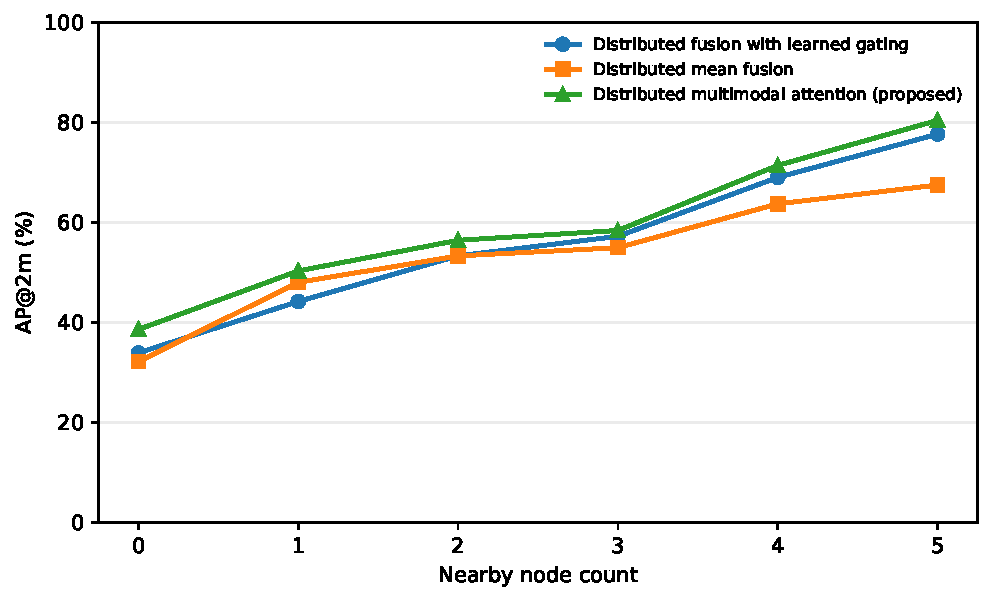
\includegraphics[width=0.90\textwidth]{paper_results/figures/fig_01_node_count_ap.pdf}
    \caption{AP@2m as the number of available nearby sensing nodes varies.}
    \label{fig:experiments-node-ap}
\end{figure}

\begin{figure}[H]
    \centering
    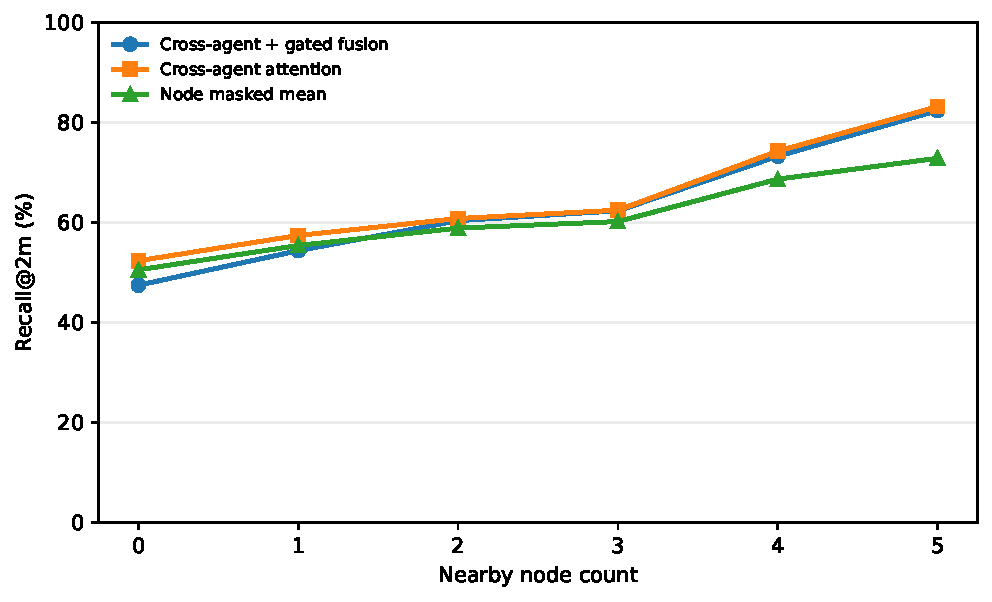
\includegraphics[width=0.90\textwidth]{paper_results/figures/fig_02_node_count_recall.pdf}
    \caption{Recall@2m as the number of available nearby sensing nodes varies.}
    \label{fig:experiments-node-recall}
\end{figure}

\begin{figure}[H]
    \centering
    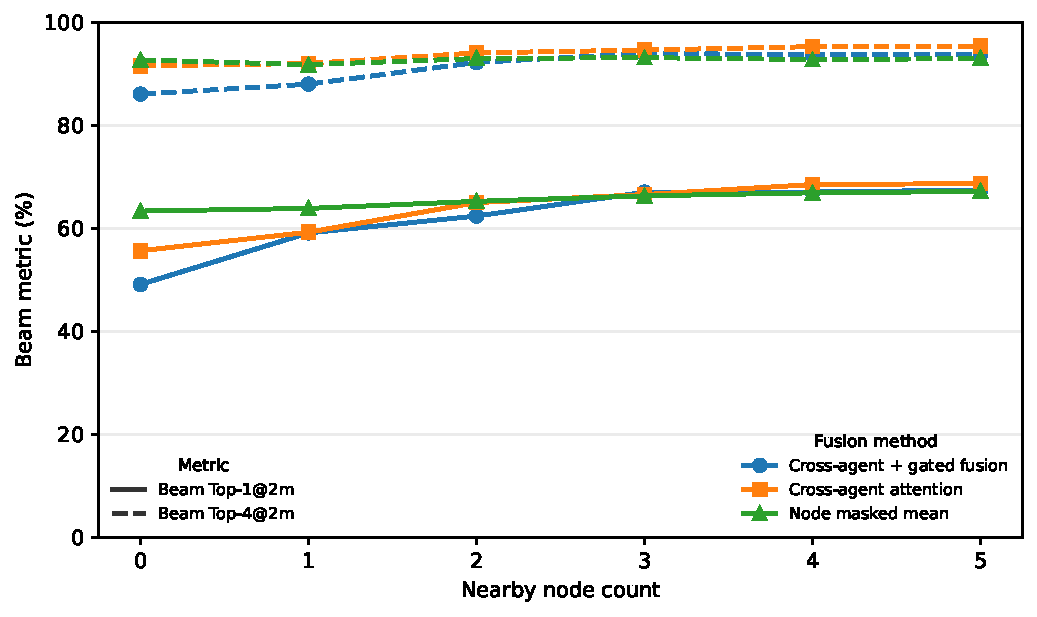
\includegraphics[width=0.90\textwidth]{paper_results/figures/fig_03_node_count_beam.pdf}
    \caption{Beam Top-1@2m and Top-4@2m as the number of available nearby
    sensing nodes varies.}
    \label{fig:experiments-node-beam}
\end{figure}

\section{Communication Performance}
\label{sec:experiments-beam-management}

\subsection{Performance Across Environmental Conditions}
\label{subsec:experiments-weather-system}

Table~\ref{tab:experiments-system-weather} and
Figure~\ref{fig:experiments-weather-rate} compare the three measurement
policies under each environmental condition.  In Clear conditions, DMSA-BM
reaches an effective user rate of \(155.453\) Mbps with \(1.39\%\) CSI-RS
overhead.  SSB-guided refinement with \(K_{\mathrm{ref}}=4\) reaches
\(151.367\) Mbps with \(1.90\%\) overhead, whereas the
\(K_{\mathrm{ref}}=12\) operating point reaches \(127.033\) Mbps with
\(5.71\%\) overhead.

The sensing-use entries and their complementary fallback ratios clarify how
the policy reaches these outcomes.  Sensing candidates are used for \(76.35\%\)
of the Clear instances, \(56.65\%\) of the Rain/Fog instances, and \(30.07\%\)
of the Night instances.  The corresponding fallback ratios are \(23.65\%\), \(43.35\%\), and
\(69.93\%\).  Thus, DMSA-BM retains SSB-guided refinement whenever no
accepted association with a currently observed track is available, instead of
applying target-indexed beam information to a VUE unconditionally.

\begin{table}[H]
    \centering
    \caption{Communication performance by environmental condition under the
    common system configuration.  The effective rate is averaged over VUEs and
    communication cycles.}
    \label{tab:experiments-system-weather}
    \small
    \renewcommand{\arraystretch}{1.10}
    \resizebox{\textwidth}{!}{%
    \begin{tabular}{llrrr}
        \toprule
        Condition & Policy & Effective rate (Mbps) &
        CSI-RS overhead (\%) & Sensing use (\%) \\
        \midrule
        Clear & SSB-guided refinement, \(K_{\mathrm{ref}}=4\) & 151.367 & 1.90 & 0.00 \\
        Clear & SSB-guided refinement, \(K_{\mathrm{ref}}=12\) & 127.033 & 5.71 & 0.00 \\
        Clear & DMSA-BM & 155.453 & 1.39 & 76.35 \\
        \addlinespace
        Rain/Fog & SSB-guided refinement, \(K_{\mathrm{ref}}=4\) & 147.571 & 1.90 & 0.00 \\
        Rain/Fog & SSB-guided refinement, \(K_{\mathrm{ref}}=12\) & 115.342 & 5.71 & 0.00 \\
        Rain/Fog & DMSA-BM & 150.801 & 1.57 & 56.65 \\
        \addlinespace
        Night & SSB-guided refinement, \(K_{\mathrm{ref}}=4\) & 127.807 & 1.90 & 0.00 \\
        Night & SSB-guided refinement, \(K_{\mathrm{ref}}=12\) & 105.294 & 5.71 & 0.00 \\
        Night & DMSA-BM & 132.743 & 1.71 & 30.07 \\
        \bottomrule
    \end{tabular}%
    }
\end{table}

\begin{figure}[H]
    \centering
    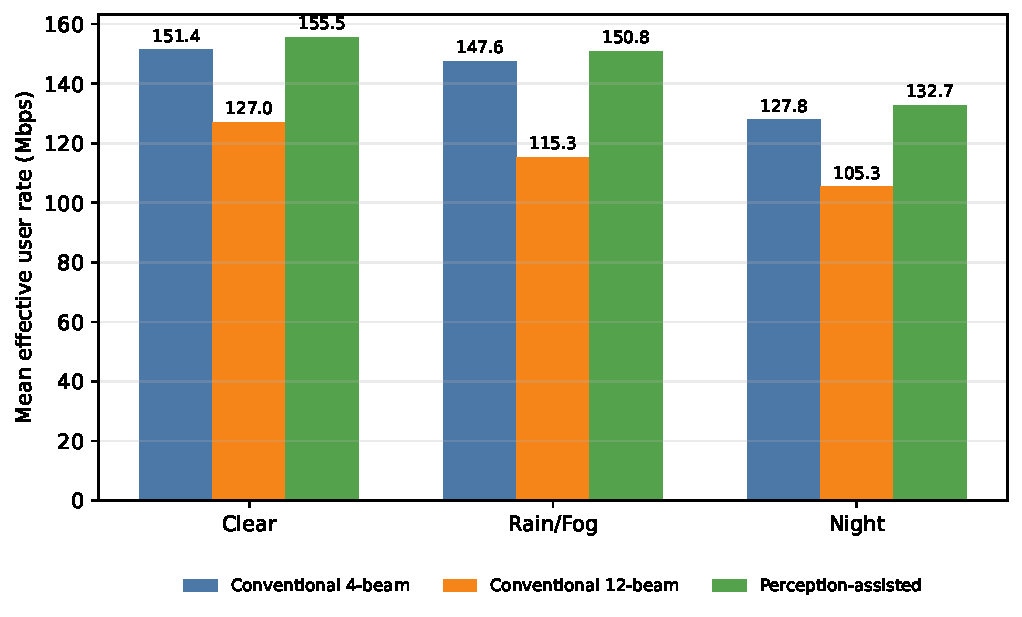
\includegraphics[width=0.88\textwidth]{paper_results/figures/fig_04_core_user_rate_by_weather.pdf}
    \caption{Effective user rate by environmental condition and measurement
    policy.}
    \label{fig:experiments-weather-rate}
\end{figure}

\subsection{Aggregate Performance}
\label{subsec:experiments-macro-system}

Figure~\ref{fig:experiments-system-tradeoff} aggregates the three environmental
conditions with equal weight.  DMSA-BM achieves an effective user rate of
\(146.332\) Mbps with \(1.56\%\) CSI-RS overhead.  The corresponding values
for SSB-guided refinement are \(142.248\) Mbps and \(1.90\%\) at
\(K_{\mathrm{ref}}=4\), and \(115.890\) Mbps and \(5.71\%\) at
\(K_{\mathrm{ref}}=12\).

DMSA-BM remains explicitly conditional.  Its aggregate sensing-use ratio is
\(54.35\%\), while \(45.65\%\) of instances use SSB-guided refinement as the
fallback.  Taken together, the rate and overhead values show
the consequence of using sensing only when a current detection and a credible
target-to-user association are available.  The service beam is still selected
from the actually measured CSI-RS candidates.

\begin{figure}[H]
    \centering
    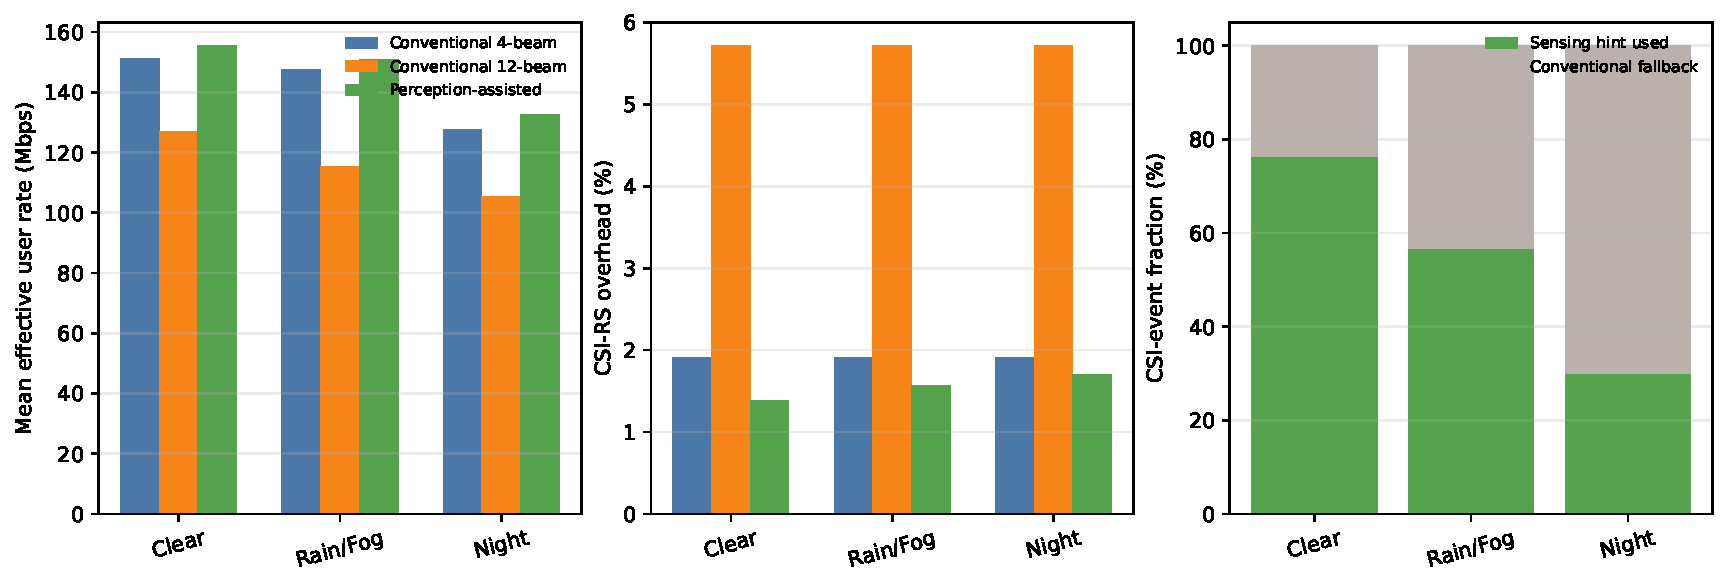
\includegraphics[width=0.96\textwidth]{paper_results/figures/fig_05_core_user_rate_hint_overhead.pdf}
    \caption{Aggregate effective rate, CSI-RS overhead, and the
    sensing-use/fallback composition under the common system configuration.}
    \label{fig:experiments-system-tradeoff}
\end{figure}

\section{Tracking Performance}
\label{sec:experiments-tracking}

\subsection{Comparison of Tracking Models}
\label{subsec:experiments-tracker-system}

Table~\ref{tab:experiments-trackers} evaluates the three trackers with the same
Top-1 CE detector and system configuration.  Their effective rates are close,
with \(146.332\) Mbps for IMM, \(146.373\) Mbps for KF-CV, and
\(145.880\) Mbps for KF-CT.  KF-CV is marginally higher than IMM in this
metric.  The table therefore does not support an effective-rate claim of
universal IMM superiority.

The sensing-use ratios are also close, at \(54.35\%\) for IMM, \(53.80\%\) for
KF-CV, and \(52.26\%\) for KF-CT.  These values show that the three trackers
operate at comparable frequencies of sensing-assisted candidate selection under
the evaluated procedure.  IMM is retained in DMSA-BM for its
multi-model state-estimation role in association maintenance.  The table should
therefore be interpreted as an end-to-end comparison rather than as a
tracker-only proof of superiority.

\begin{table}[H]
    \centering
    \caption{Aggregate communication results for the tracker variants under
    the common detector and system configuration.}
    \label{tab:experiments-trackers}
    \small
    \begin{tabular}{lrr}
\toprule
Tracker & Mean effective user rate (Mbps) & Sensing use (\%) \\
\midrule
IMM & 146.332 & 54.35 \\
KF-CV & \textbf{146.373} & 53.80 \\
KF-CT & 145.880 & 52.26 \\
\bottomrule
\end{tabular}

\end{table}

\section{Discussion and Limitations}
\label{sec:experiments-discussion}

The results support a consistent evidence chain.  Multimodal and nearby-node
observations improve different aspects of target availability and beam ranking;
association acceptance and current-track observation determine whether this
evidence is converted into a narrower CSI-RS measurement action; and the system
evaluation reports the resulting effective throughput together with the
associated measurement cost.  The substantial fallback share under Rain/Fog
and Night is therefore an integral part of DMSA-BM and should be interpreted
together with the average-rate result.

The system analysis characterises association-mediated operation through the
sensing-use ratio, fallback ratio, and average effective user rate; accepted-association
accuracy, lower-tail rate, and outage are outside the reported analysis.  The
conclusions are further limited to a local target-BS service region, a simulated
multimodal dataset, approximately 100-ms ray-tracing channel segments, and the
stated RZF and resource model.  They therefore describe performance under the
specified system assumptions rather than a complete 5G NR protocol stack or a
direct real-world deployment.
